\chapter{Quaternions}
This chapter presents a primer on quaternions so the reader can understand the theory developed in the research section.
The quaternions are a number system that extends the complex numbers. 
They were first described by Irish mathematician William Rowan Hamilton in 1843 and applied to mechanics in three-dimensional space. 
In modern mathematical language, quaternions form a four-dimensional associative normed division algebra over the real numbers, and therefore also a domain.
In this chapter we will define operations on the quaternion algebra, draw connection to the complex numbers and $\mathbb{R}^3$, and show some real world use cases of quaternions.


\section{Quaternion Algebra}\label{s:quatalg}
In 1833 Hamilton proposed that complex numbers $\mathbb{C}$ be defined as the set $\mathbb{R}^2$ of ordered pairs $(a, b)$ of real numbers.
He then began working to see if triplets $(a,b,c)$ could extend multiplication of complex numbers.
In 1843 he discovered a way to multiply in four dimensions instead of three, but the multiplication lost commutativity.
This construction is now known as quaternions.
Quaternions are composed of four components, one real part, and three imaginary parts.
Typically denoted as
\begin{equation}
\mathbb{H} = \{a + b\textit{i} + c\textit{j} + d\textit{k}~:~a,b,c,d \in \mathbb{R}\}
\label{eq:quaternion1}
\end{equation}
where $a$ is the real part, $(i,j,k)$ denotes the three imaginary axis, and $(b,c,d)$ denotes the three imaginary components.
Sometimes $a$ is referred to as the scalar part and $(b,c,d)$ as the vector part.
Note that we shall use the forms $bi + cj + dk$ and $(b,c,d)$ interchangeably.
Quaternions are governed by the following arithmetic:
\begin{equation}
i^2=j^2=k^2=ijk=-1
\label{eq:quarternion2}
\end{equation}
which leads to the non-commutative multiplication rules
\begin{equation}
ij=k,~jk=i,~ki=j,~ji=-k,~kj=-i,~ik=-j
\label{eq:quarternion3}
\end{equation}


\subsection{Addition and Multiplication}
The addition of two quaternions acts component wise, exactly the same as two complex numbers.
Consider the quaternion $q$
\begin{equation}
q = q_0 + q_1\textit{i} + q_2\textit{j} + q_3\textit{k}
\label{eq:q}
\end{equation}
and the quaternion $p$
\begin{equation}
p = p_0 + p_1\textit{i} + p_2\textit{j} + p_3\textit{k}.
\label{eq:p}
\end{equation}
Their addition is given by
\begin{equation}
p + q = (p_0+q_0) + (p_1+q_1)\textit{i} + (p_2+q_2)\textit{j} + (p_3+q_3)\textit{k}.
\label{eq:quataddition}
\end{equation}

The product of two quaternions will produce another quaternion and is given by
\begin{align*}
pq &= (p_0 + p_1\textit{i} + p_2\textit{j} + p_3\textit{k})(q_0 + q_1\textit{i} + q_2\textit{j} + q_3\textit{k}) \nonumber \\
&= p_0q_0 - (p_1q_1 + p_2q_2 + p_3q_3) \nonumber \\
&~~~ + p_0(q_1\textit{i} + q_2\textit{j} + q_3\textit{k}) + q_0(p_1\textit{i} + p_2\textit{j} + p_3\textit{k}) \nonumber \\
&~~~ + (p_2q_3 - p_3q_2)\textit{i} + (p_3q_1 - p_1q_3)\textit{j} + (p_1q_2p - p_2q_1)\textit{k}. \nonumber
\end{align*}
It can be seen that the result is a quaternion by refactoring it, which we do by utilizing the inner and cross products of two vectors in $\mathbb{R}^3$ \cite{hungerford1980algebra}:
\begin{equation}
pq = p_0q_0 - \textbf{p}\cdot\textbf{q} + p_0\textbf{q} + q_0\textbf{p} + \textbf{p} \times \textbf{q}
\label{eq:quatmult}
\end{equation}
where $\textbf{p} = (p_1,p_2,p_3)$ and $\textbf{q} = (q_1,q_2,q_3)$ are the vector parts of $p$ and $q$ respectively.
The first two terms form the scalar part and the last three form the vector part.


\subsection{Conjugate, Norm, and Inverse}
The \textit{conjugate} of $q$, denoted as $q^*$, is defined as a negation of the vector part of $q$
\begin{equation}
q^* = q_0 - \textbf{q}
\label{eq:quatconjugate}
\end{equation}
and has the properties
\begin{align*}
(q^*)^* &= q_0 - (-\textbf{q}) = q, \\
q + q^* &= 2q_0, \\
q^*q &= (q_0 - \textbf{q})(q_0 + \textbf{q}) \\
&= q_0q_0 - (-\textbf{q}) \cdot \textbf{q} + q_0\textbf{q} + (-\textbf{q})q_0 + (-\textbf{q}) \times \textbf{q} \\
&= q_0^2 + \textbf{q} \cdot \textbf{q} \\
&= q_0^2 + q_1^2 + q_2^2 + q_3^2 \\
&= qq^*
\end{align*}

The \textit{norm} of a quaternion $q$, denoted as $|q|$, is the scalar
\begin{equation*}
|q| = \sqrt{q^*q}
\label{eq:quatnorm}
\end{equation*}
and a quaternion is said to be a \textit{unit quaternion} if its norm is 1.
For instance let $\mathbf{\hat{u}} = u_1i+u_2j+u_3k$ be any unit vector, then a unit quaternion is given by
\begin{equation*}
q_{unit} = \mbox{cos}\theta + \mathbf{\hat{u}}~\mbox{sin}\theta.
\end{equation*}
One can check by plugging this into \eqref{eq:quatnorm}
\begin{align*}
|q_{unit}| &= \sqrt{q_{unit}^* q_{unit}} \\
&= \sqrt{\mbox{cos}^2\theta + u_1~\mbox{sin}^2\theta + u_2~\mbox{sin}^2\theta + u_3~\mbox{sin}^2\theta} \\
&= \sqrt{\mbox{cos}^2\theta + \mbox{sin}^2\theta} \\
&= 1.
\end{align*}

The norm of the product of two quaternions $p$ and $q$ is the product of the individual norms,
\begin{align*}
|pq|^2 &= (pq)(pq)^* \\
&= pqq^*p^* \\
&= p|q|^2p^* \\
&= pp^*|q|^* \\
&= |p|^* |q|^*.
\end{align*}

The \textit{inverse} of a quaternion $q$ is defined as 
\begin{equation*}
q^{-1} = \frac{q^*}{|q|^2},
\end{equation*}
which gives $q^{-1}q = qq^{-1} = 1.$
For all unit quaternions, the inverse is equal to the conjugate.


\section{Geometric Representation of Quaternions}
Here we will try to show a more intuitive geometric interpretation of quaternions by showing their link to complex numbers and how they can be used to represent rotations.
To do this we will first give a brief reminder of complex numbers and their geometric interpretation of rotating a 2D plane.

\subsection{Complex Algebra}
Complex numbers are composed of two components, one real part, and one imaginary part.
This is usually denoted as
\begin{equation}
\mathbb{C} = \{a + bi~:~a,b \in \mathbb{R}, ~~i^2=-1\}
\label{eq:complexalgebra}
\end{equation}
where $a$ is the real part, $i$ denotes the single imaginary axis, and $b$ denotes the single imaginary component.

Let $c$ and $d$ be two complex numbers, their addition is given by
\begin{equation}
c + d = (c_0 + c_1i) + (d_0 + d_1i) = (c_0+d_0) + (c_1+d_1)i
\label{eq:complexaddition}
\end{equation}
and their multiplication by
\begin{equation}
cd = (c_0d_0 - c_1d_1) + (c_0d_1 + c_1d_0)i.
\label{eq:complexmult}
\end{equation}
Any complex number has a length given by
\begin{equation}
|c| = |c_0+c_1i| = \sqrt{c_0^2 + c_1^2}
\label{eq:complexlength}
\end{equation}
and like quaternions, any complex number with a length of 1 is called a \textit{unit complex number}.


\subsection{Complex Rotation Operation}
The set of unit complex numbers lies on the unit circle in $\mathbb{C}$ and Leonhard Euler showed that
\begin{equation}
e^{i\theta} = \mbox{cos}~\theta + i~\mbox{sin}~\theta.
\label{eq:euler}
\end{equation}
If we multiply this by any positive number $r$, we get a complex number of length $r$.
Therefore, by adjusting the length $r$ and the angle $\theta$, we can write any complex number.
This form goes by the name \textit{polar coordinates}.

They are a great way to multiply complex numbers. 
Instead of \eqref{eq:complexmult} let us write each complex in polar coordinates
\begin{equation*}
c = (c_0+c_1i) = re^{i\theta}, ~~~d = (d_0+d_1i) = se^{i\phi}
\end{equation*}
and then multiply
\begin{equation*}
cd = re^{i\theta}se^{i\phi} = rse^{i(\theta+\phi)}.
\end{equation*}
This tells us that to multiply two complex numbers, multiply their lengths and add their angles.
In particular, if we multiply a given complex number by a unit complex number the resulting length is the same, but we have rotated it by $\theta$ degrees. 
This gives us some hints that quaternions may also be able to perform rotation operation in higher dimensional space.



\subsection{Quaternion Rotation Operation}
We will stick to interpretations of quaternions in $\mathbb{R}^3$ as it is easier to visualize, but how can a quaternion, which exists in $\mathbb{R}^4$, operate on a 3D vector?
Recall that the imaginary components of a quaternion are called the vector part and a vector $\textbf{v} \in \mathbb{R}^3$ is a \textit{pure quaternion} whose real part is zero.

\begin{figure*}[!h]
	\centering
		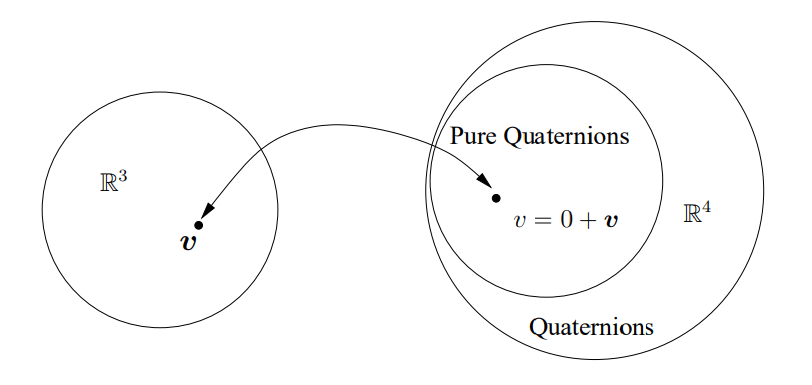
\includegraphics[width=1.0\textwidth]{figures/r3.png}
	\caption{$\mathbb{R}^3$ can be viewed as a subspace of quaternions called pure quaternions which have a real part of zero. \cite{jia2008quaternions}}
	\label{f:r3}
\end{figure*}

Using the unit quaternion $q$ let us define a function $L_q:~\mathbb{R}^3 \rightarrow \mathbb{R}^3$ on vectors $\textbf{v} \in \mathbb{R}^3$ \cite{hungerford1980algebra}:
\begin{align}
L_q(\textbf{v}) &= q\textbf{v}q^* \nonumber \\
&= (q_0^2 - ||\textbf{q}||^2)\textbf{v} + 2(\textbf{q}\cdot\textbf{v})\textbf{q} + 2q_0(\textbf{q} \times \textbf{v}). 
\label{eq:Lq}
\end{align}

Two observations to note are that first, the operation \eqref{eq:Lq} does not modify the length of the vector $\textbf{v}$:
\begin{align*}
||L_q(\textbf{v})|| &= ||q\textbf{v}q^*||  \\
&= |q| \cdot ||\textbf{v}|| \cdot |q^*| \\
&= ||\textbf{v}||. 
\end{align*}
And second, the direction of $\textbf{v}$, if along $\textbf{q}$, is left unchanged by the function. To verify let $\textbf{v} = k\textbf{q}$
\begin{align*}
L_q(\textbf{v}) &= q(k\textbf{q})q^*  \\
&= (q_0^2 - ||\textbf{q}||^2)k\textbf{q} + 2(\textbf{q}\cdot k\textbf{q})\textbf{q} + 2q_0(\textbf{q} \times k\textbf{q}) \\
&= k(q_0^2 + ||\textbf{q}||^2)\textbf{q} \\
&= k\textbf{q}.
\end{align*}
Using our insights from complex numbers this lets us guess that the function \eqref{eq:Lq} acts like a rotation about $\textbf{q}$.

\begin{theorem}
For any unit quaternion
\begin{equation}
q = q_0 + \textbf{q} = \mbox{cos}\frac{\theta}{2} + \mathbf{\hat{u}}\mbox{sin}\frac{\theta}{2},
\label{eq:unitquat}
\end{equation}
where $\mathbf{\hat{u}} = u_1i+u_2j+u_3k$ is any unit vector and for any vector $\textbf{v} \in \mathbb{R}^3$ the result of the function
\begin{equation*}
L_q(\textbf{v}) = q\textbf{v}q^*
\end{equation*}
on $\textbf{v}$ is equivalent to a rotation of the vector through an angle $\theta$ about $\mathbf{\hat{u}}$ as the axis of rotation.
\end{theorem}

\begin{proof}
Given a vector $\textbf{v} \in \mathbb{R}^3$, we decompose it as $\textbf{v} = \textbf{a} + \textbf{n}$, where $\textbf{a}$ is the component along the vector $\textbf{q}$ and $\textbf{n}$ is the component normal to $\textbf{q}$. 
Then we show that under the function $L_q$, $\textbf{a}$ is invariant, while $\textbf{n}$ is rotated about $\textbf{q}$ through an angle $\theta$. 

Earlier we showed that $\textbf{a}$ is invariant under $L_q$ so let us see how $L_q$ transforms $\textbf{n}$.
\begin{align*}
L_q(\textbf{n}) &= (q_0^2 - ||\textbf{q}||^2)\textbf{n} + 2(\textbf{q} \cdot \textbf{n})\textbf{q} + 2q_0(\textbf{q} \times \textbf{n}) \\
&= (q_0^2 - ||\textbf{q}||^2)\textbf{n} + 2q_0(\textbf{q} \times \textbf{n}) \\
&= (q_0^2 - ||\textbf{q}||^2)\textbf{n} + 2q_0||\textbf{q}||(\mathbf{\hat{u}} \times \textbf{n}),
\end{align*}
where in the last step we introduced $\mathbf{\hat{u}} = \textbf{q}/||\textbf{q}||$.
Let $\textbf{n}_{\bot} = \mathbf{\hat{u}} \times \textbf{n}$ to get
\begin{equation}
L_q(\textbf{n}) = (q_0^2 -||\textbf{q}||^2)\textbf{n} + 2q_0||\textbf{q}||\textbf{n}_{\bot}.
\label{eq:p11}
\end{equation}
Also note that $\textbf{n}_{\bot}$ and $\textbf{n}$ have the same length:
\begin{equation*}
||\textbf{n}_{\bot}|| = ||\textbf{n} \times \mathbf{\hat{u}}|| = ||\textbf{n}|| \cdot ||\mathbf{\hat{u}}||\mbox{sin}\frac{\pi}{2} = ||\textbf{n}||.
\end{equation*}
Then rewriting \eqref{eq:p11} we arrive at
\begin{align*}
L_q(\textbf{n}) &= \left( \mbox{cos}^2 \frac{\theta}{2} - \mbox{sin}^2 \frac{\theta}{2} \right) \textbf{n} + \left( 2\mbox{cos} \frac{\theta}{2} \mbox{sin} \frac{\theta}{2} \right) \textbf{n}_{\bot} \\
&= \mbox{cos}~\theta \textbf{n} + \mbox{sin}~\theta \textbf{n}_{\bot}.
\end{align*}
The resulting vector is a rotation of $\textbf{n}$ through an angle $\theta$ in the plane defined by $\textbf{n}$ and $\textbf{n}_{\bot}$ \cite{jia2008quaternions}.
\end{proof}


\section{Conclusion}\label{s:quatConc}
In this chapter we gave the reader the needed information of the quaternion algebra for theory sections to follow.
We have discussed some motivation for the representational power of quaternions by showing how they can encode rotations in a compact form.
It was also hinted that the structure of quaternion algebra benefits CNNs specifically.
This comes from the multiplication rule for quaternions, which makes the convolution operation in the CNN treat the channels of the image as a single entity. 
We will show this in detail in the next chapter within the quaternion convolution Section \ref{s:qc}.
















